\bookchapter{Ownership and Borrowing}\label{ch:rust3}

\section*{Explanation}
This is the chapter that makes Rust different, and the one that people find hardest. It answers a question that Python hides from you: \emph{who is responsible for a piece of memory, and when is it freed?} The answer of Rust is a simple set of rules that the compiler checks. If you follow them, you get a program without memory errors and without a garbage collector. If you do not, the compiler tells you, and tells you where.

\section*{Stack and heap}
A running program uses two kinds of memory. The \textbf{stack} is a fast, tidy memory for values whose size is known when the program is compiled (an \verb!i32!, an \verb!f64!, an array of three numbers, a pair of coordinates): each function call puts its variables on top of the stack, and they vanish when the function returns. The \textbf{heap} is for values whose size is only known while running or that must live longer: a text that grows, a list that gets more elements, a camera image. The program asks for a piece of the heap, receives its address and must give it back when it is finished. A \verb!Vec<f64>! therefore consists of a small \emph{handle} on the stack (address, length, capacity) and the numbers on the heap.
\begin{center}
\begin{tikzpicture}[>={Stealth[length=2.2mm]},font=\footnotesize]
 \node[font=\bfseries\footnotesize] at (1.3,2.5) {stack};
 \node[font=\bfseries\footnotesize] at (8.3,2.5) {heap};
 \draw[thick] (0,0) rectangle (2.6,2.2);
 \draw (0,1.65) -- (2.6,1.65); \draw (0,1.1) -- (2.6,1.1); \draw (0,0.55) -- (2.6,0.55);
 \node at (1.3,1.93) {\texttt{x = 42}};
 \node at (1.3,1.375) {\texttt{y = 3.5}};
 \node[align=center] at (1.3,0.82) {\texttt{v}: address};
 \node at (1.3,0.27) {\texttt{v}: len 4, cap 4};
 \draw[thick] (6.4,0.7) rectangle (10.4,1.5);
 \foreach \i/\t in {0/3.0,1/1.0,2/2.0,3/5.0} {
   \draw (6.4+\i,0.7) rectangle (7.4+\i,1.5); \node at (6.9+\i,1.1) {\t};}
 \draw[->,thick] (2.6,0.82) -- (6.4,1.1);
 \node[gray,align=left,anchor=west] at (3.0,2.05) {fixed size, automatic};
 \node[gray,align=left,anchor=west] at (6.4,0.3) {size chosen while the program runs};
\end{tikzpicture}
\captionof{figure}{A \texttt{let v = vec![3.0, 1.0, 2.0, 5.0];} puts a small handle on the stack and the numbers on the heap.}
\end{center}
In Python \emph{all} objects live on the heap, and the interpreter counts how many names refer to each object and frees it when the count reaches zero (plus a garbage collector for cycles). In C you call \verb!malloc! and \verb!free! yourself, and every forgotten or doubled \verb!free! is a bug. Rust uses a third way.

\section*{The three rules}
\begin{keyidea}[The ownership rules]
(1) Every value has exactly one \textbf{owner}, a variable. (2) There is only one owner at a time. (3) When the owner goes out of scope, the value is \textbf{dropped} (freed) automatically, at the closing brace.
\end{keyidea}
%rsmain:scope
\begin{verbatim}
    {
        let v = vec![1, 2, 3];       // v owns the heap memory
        println!("{:?}", v);
    }                                // v ends here: memory is freed
\end{verbatim}
No \verb!free! call and no counter: the compiler inserts the freeing at the closing brace. The same mechanism closes files, network sockets and mutex locks, which is why Rust programs rarely forget to do so.

\section*{Moves}
What happens when you assign a vector to another variable?
%rsfail:moved
\begin{verbatim}
fn main() {
    let a = vec![1, 2, 3];
    let b = a;                 // the ownership MOVES to b
    println!("{:?}", a);       // error: a is no longer valid
}
\end{verbatim}
In Python both names would refer to the same list. If Rust did the same, both would try to free the memory at the end (a ``double free''), or one would use it after the other freed it. So Rust \textbf{moves} the ownership: \verb!b! is the new owner, \verb!a! is not usable any more, and the compiler says \verb!error[E0382]: borrow of moved value: `a`!. Only the small handle is copied, the numbers on the heap stay where they are:
\begin{center}
\begin{tikzpicture}[>={Stealth[length=2.2mm]},font=\footnotesize]
 \node at (1.0,2.3) {\textbf{before} \texttt{let b = a;}};
 \draw[thick] (0,1.0) rectangle (2.0,1.8); \node at (1.0,1.4) {\texttt{a}};
 \draw[thick,fill=gray!15] (4.2,1.0) rectangle (6.6,1.8); \node at (5.4,1.4) {\texttt{1 2 3}};
 \draw[->,thick] (2.0,1.4)--(4.2,1.4);
 \node at (9.3,2.3) {\textbf{after}};
 \draw[thick,dashed,gray] (7.4,1.0) rectangle (9.4,1.8); \node[gray] at (8.4,1.4) {\texttt{a}};
 \draw[thick] (7.4,-0.3) rectangle (9.4,0.5); \node at (8.4,0.1) {\texttt{b}};
 \draw[thick,fill=gray!15] (11.0,0.3) rectangle (13.4,1.1); \node at (12.2,0.7) {\texttt{1 2 3}};
 \draw[->,thick] (9.4,0.1)--(11.0,0.6);
 \node[gray] at (8.4,2.0) {\scriptsize moved: unusable};
\end{tikzpicture}
\captionof{figure}{A move transfers the ownership; the data does not move at all.}
\end{center}
Passing a value to a function is also a move:
%rsfail:moved_fn
\begin{verbatim}
fn consume(v: Vec<i32>) -> usize { v.len() }

fn main() {
    let a = vec![1, 2, 3];
    let n = consume(a);        // a moves into the function
    println!("{n} {:?}", a);   // error: a was moved
}
\end{verbatim}
Two ways out: you can give the value back (return it) or let the function only \emph{borrow} it, the usual way, described next. And a third: \verb!let b = a.clone();! makes a real, independent copy of the data (a new allocation), explicit and visible, so you notice when you spend time and memory on copying.
\begin{keyidea}[Copy types]
Simple values that live completely on the stack (\verb!i32!, \verb!f64!, \verb!bool!, \verb!char!, tuples and arrays of them) are copied instead of moved: after \verb!let y = x;! with \verb!x: i32! both are valid. They have the property \textbf{Copy}.
\end{keyidea}

\section*{Borrowing: references}
A function that only wants to \emph{look} at a vector should not take it away. It receives a \textbf{reference}, written \verb!&!: ``I borrow this and give it back''.
%rs:borrow
\begin{verbatim}
fn total(xs: &Vec<f64>) -> f64 {
    xs.iter().sum()
}

fn main() {
    let d = vec![1.5, 2.5, 3.0];
    let s = total(&d);                // lend d
    println!("{s} {:?}", d);          // d is still ours
}
\end{verbatim}
prints \verb!7 [1.5, 2.5, 3.0]!. A reference gives read access only. To change the data you borrow \emph{mutably} with \verb!&mut!, and the owner must be declared \verb!mut!:
%rs:borrow_mut
\begin{verbatim}
fn scale(xs: &mut Vec<f64>, k: f64) {
    for x in xs.iter_mut() {
        *x *= k;                      // * : follow the reference
    }
}

fn main() {
    let mut d = vec![1.0, 2.0];
    scale(&mut d, 10.0);
    println!("{:?}", d);              // [10.0, 20.0]
}
\end{verbatim}
\begin{keyidea}[The borrowing rules]
At any moment you may have \emph{either} any number of shared references (\verb!&T!, read only) \emph{or} exactly one mutable reference (\verb!&mut T!), and never both. References must never outlive the value they point to.
\end{keyidea}
This is the rule that gives Rust its safety: ``many readers or one writer'' is exactly the condition that avoids a data race (two threads, one writing while the other reads, Chapter~\ref{ch:rust6}), and the same rule avoids the single-threaded bug of changing a list while you walk through it.
%rsfail:two_mut
\begin{verbatim}
fn main() {
    let mut v = vec![1, 2, 3];
    let first = &v[0];         // shared borrow
    v.push(4);                 // mutable borrow: error
    println!("{first}");
}
\end{verbatim}
Here \verb!push! may move the numbers to a bigger piece of heap memory, and \verb!first! would then point into freed memory (a \emph{dangling} pointer). The compiler refuses: \verb!error[E0502]: cannot borrow `v` as mutable because it is also borrowed as immutable!. If you use \verb!first! \emph{before} the push, the program compiles: a borrow lasts only until its last use.
\begin{center}
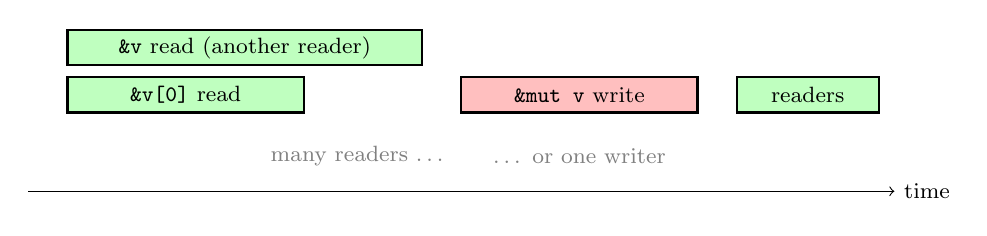
\begin{tikzpicture}[font=\footnotesize]
 \draw[->] (0,0)--(11,0) node[right]{time};
 \draw[thick,fill=green!25] (0.5,1.0) rectangle (3.5,1.45); \node at (2,1.22) {\texttt{\&v[0]} read};
 \draw[thick,fill=green!25] (0.5,1.6) rectangle (5.0,2.05); \node at (2.75,1.82) {\texttt{\&v} read (another reader)};
 \draw[thick,fill=red!25] (5.5,1.0) rectangle (8.5,1.45); \node at (7,1.22) {\texttt{\&mut v} write};
 \draw[thick,fill=green!25] (9.0,1.0) rectangle (10.8,1.45); \node at (9.9,1.22) {readers};
 \node[gray,align=center] at (4.2,0.45) {many readers \ldots};
 \node[gray,align=center] at (7,0.45) {\ldots\ or one writer};
\end{tikzpicture}
\captionof{figure}{Readers and writers never overlap in time. The compiler checks that for you.}
\end{center}

\section*{Strings: \texttt{String} and \texttt{\&str}}
Text comes in two kinds. A \verb!String! owns its characters on the heap and can grow, like a Python \verb!str! that you may extend. A \verb!&str! (a ``string slice'') is a borrowed view on text that lives somewhere else; a literal \verb!"hello"! is a \verb!&str! that lives inside the program. A function that only reads text should take a \verb!&str!, because both kinds can be passed to it.
%rs:strings
\begin{verbatim}
fn shout(s: &str) -> String {
    s.to_uppercase() + "!"
}

fn main() {
    let mut name = String::from("robot");   // owned, growable
    name.push_str("-7");
    let part: &str = &name[0..5];           // a slice: borrowed
    println!("{name} {part} {}", shout(part));
    println!("{}", shout("kick"));
    println!("{}", name.len());
}
\end{verbatim}
prints \verb!robot-7 robot ROBOT!!, \verb!KICK!! and \verb!7!. Text is stored as UTF-8, so a slice must start and end at character borders (an index inside a multi-byte character panics) and you cannot index a string with a single number (\verb!name[0]! is an error); use \verb!name.chars().nth(0)! or slices of bytes when you know the text is plain ASCII.

\section*{Slices}
A \textbf{slice} \verb!&[T]! is a borrowed view on a part of an array or vector, a pointer and a length. It is the preferred parameter type for read-only access to sequences, as in Chapter~\ref{ch:rust2}: \verb!fn mean(xs: &[f64])! accepts a whole \verb!Vec!, an array, or a part of them.
%rsmain:slices
\begin{verbatim}
    let v = vec![10, 20, 30, 40, 50];
    let mid = &v[1..4];            // [20, 30, 40]
    let tail = &v[3..];            // [40, 50]
    println!("{:?} {:?} {}", mid, tail, mid.len());
    let (left, right) = v.split_at(2);
    println!("{:?} {:?}", left, right);
\end{verbatim}
prints \verb![20, 30, 40] [40, 50] 3! and \verb![10, 20] [30, 40, 50]!. The slice of a vector borrows the vector, so the borrowing rules apply.

\section*{Lifetimes}
Every reference has a \textbf{lifetime}: the part of the program in which it is valid. Usually the compiler works it out and you never write it. It asks for help when a function returns a reference and could return one of several of its parameters:
%rs:lifetime
\begin{verbatim}
fn longer<'a>(a: &'a str, b: &'a str) -> &'a str {
    if a.len() >= b.len() { a } else { b }
}

fn main() {
    let x = String::from("kick off");
    let r;
    {
        let y = String::from("goal");
        r = longer(&x, &y).len();     // fine: only the length survives
    }
    println!("{r}");
}
\end{verbatim}
prints \verb!8!. The \verb!'a! says: ``the returned reference is valid as long as \emph{both} arguments are''. If you tried to keep the returned reference itself after \verb!y! is gone, the compiler would stop you with \verb!error[E0597]: `y` does not live long enough!. Lifetimes are not new runtime information, they exist only for the compiler. When you meet them in real code, read \verb!'a! as ``some region of the program'', and fix errors by returning an owned value (\verb!String!) instead of a reference.

\section*{Robot example: a camera frame}
A frame has $640\times480\times3$ bytes, about $0.9$\,MB. Copying it for every consumer would waste time. With ownership you see in the signature what happens:
%rs:frame
\begin{verbatim}
struct Frame { data: Vec<u8>, width: usize, height: usize }

fn brightness(f: &Frame) -> f64 {            // only reads: borrows
    let sum: u64 = f.data.iter().map(|&b| b as u64).sum();
    sum as f64 / f.data.len() as f64
}

fn darken(f: &mut Frame) {                   // changes it: borrows mutably
    for b in f.data.iter_mut() { *b /= 2; }
}

fn archive(f: Frame) -> usize {              // takes it: owner changes
    f.data.len()                              // f is dropped here
}

fn main() {
    let n = 640 * 480 * 3;
    let mut f = Frame { data: vec![100; n], width: 640, height: 480 };
    println!("{}", brightness(&f));
    darken(&mut f);
    println!("{}", brightness(&f));
    println!("{}", archive(f));
}
\end{verbatim}
prints $100$, $50$ and $921600$ (the size of the data in bytes; the compiler also warns that the fields \verb!width! and \verb!height! are never read, which is true for this small example). The three signatures are three promises: \verb!&Frame! \emph{reads}, \verb!&mut Frame! \emph{may change}, \verb!Frame! \emph{takes over, the caller can never use it again}. In a larger system you read the types of the functions like a contract.

\begin{aibox}[Fighting the borrow checker]
Everyone fights the compiler at first. A few tricks that solve most cases: borrow (\verb!&!) instead of moving; end a borrow early by using the data sooner; use \verb!.clone()! while learning if a copy is cheap; return owned values; split a big struct into smaller ones that are borrowed separately. If all else fails, ask what the \emph{rule} protects: there is nearly always a real bug behind the message.
\end{aibox}

\section*{Practice problems}
\begin{enumerate}[label=\textbf{\thechapter.\arabic*}]
  \item Which of these types are \emph{Copy} (and therefore are copied on assignment), and which are moved? \verb!i64!, \verb!String!, \verb!Vec<u8>!, \verb!(f64, f64)!, \verb![i32; 4]!, \verb!&str!, \verb!bool!.
  \item The code \verb|let s = String::from("a"); let t = s; println!("{s}");| does not compile. Explain why in terms of the ownership rules, and give two corrected versions.
  \item Write a function \verb!fn count_above(xs: &[f64], limit: f64) -> usize! that counts the values above the limit, and call it with a vector and with only the second half of it. Why does the vector remain usable after the call?
  \item Write \verb!fn clamp_all(xs: &mut [f64], lo: f64, hi: f64)! that limits all values to $[lo,hi]$ in place. Test with $[-2,0.5,3]$ and $[-1,1]$.
  \item The following code does not compile. Find the line that violates the borrowing rules, and fix it in two different ways. \verb|let mut v = vec![1, 2, 3]; let r = &v; v.push(4); println!("{:?}", r);|
  \item What does the signature \verb!fn process(f: Frame)! promise compared with \verb!fn process(f: &Frame)! and \verb!fn process(f: &mut Frame)!? Which one would you choose for a function that computes the mean colour, one that blurs the picture in place, and one that sends the picture to a logging thread (which stores it)?
  \item Why can \verb!&str! be used as a parameter for both a \verb!String! and a literal, but \verb!String! as a parameter cannot? What does a caller have to do to pass a \verb!&str! to a function that wants a \verb!String!?
  \item What is a dangling reference? Show a small program in which a function tries to return a reference to a local variable, and say what the compiler reports. How do you fix it?
  \item A \verb!Vec! of ten million \verb!f64! numbers is passed in a loop to a function once per iteration. Compare the costs of passing it by value with a \verb!.clone()!, by value as a move, and by reference. Which one is the right choice if the function only reads?
  \item[\textbf{\thechapter.10}$\star$] Write a function \verb!fn split_pair(xs: &mut [f64]) -> (&mut [f64], &mut [f64])! that splits a slice at the middle (use \verb!split_at_mut!). Then change the first half to $0$ and double the second half, and print the vector. Why does Rust allow two mutable references here although the rule says only one? (Think about what the rule protects.)
\end{enumerate}
